\documentclass{article} % For LaTeX2e
\newcommand{\argmin}{\arg\!\min}
\usepackage{mathtools}
\usepackage{amsmath}

\usepackage{graphicx}
\usepackage{epstopdf} %%package to overcome problem with eps in pdf files



\DeclarePairedDelimiter\ceil{\lceil}{\rceil}

\usepackage{nips14submit_e,times}
\usepackage{hyperref}
\usepackage{url}
%\usepackage[top=5mm]{geometry}
\usepackage[ bibstyle=numeric,, maxnames=1, backend=bibtex]{biblatex}
\addbibresource{ml_project.bib}
%\documentstyle[nips14submit_09,times,art10]{article} % For LaTeX 2.09


\title{A Supervised Learning Based Approach for block page Detection}

\author{
Arian Akhavan Niaki\\
College of Information and Computer Sciences\\
University of Massachusetts\\
140 Governors Dr., Amherst, MA 01003 \\
\texttt{arian@cs.umass.edu} \\
}
% The \author macro works with any number of authors. There are two commands
% used to separate the names and addresses of multiple authors: \And and \AND.
%
% Using \And between authors leaves it to \LaTeX{} to determine where to break
% the lines. Using \AND forces a linebreak at that point. So, if \LaTeX{}
% puts 3 of 4 authors names on the first line, and the last on the second
% line, try using \AND instead of \And before the third author name.

%\newcommand{\fix}{\marginpar{FIX}}
%\newcommand{\new}{\marginpar{NEW}}

%\nipsfinalcopy % Uncomment for camera-ready version

\begin{document}
\maketitle

\begin{abstract}
Current supervised learning approaches in machine learning literature have mostly concentrated on a single aspect data such as images or text, in which they use this data to train their neural network. However, combining these two data could improve performance in the case of missing data in either images or text. In this paper, we design and implement a deep convolutional neural network which takes both the images and text data in order to do block page detection. We compare our results to ... .We show that our model achieves X 
\end{abstract}
\section{Introduction}
Extensive work has been done in supervised and unsupervised learning on both image and text classification. However, to the best of our knowledge, there does not exist an approach that applies supervised learning on a data set containing both images and textual data. This can be advantageous in the case where we either have missing data in the images or text. We see this case occurring in the field of Internet censorship and Tor discrimination.\\
Internet censorship often manifests in the form of \emph{blocked webpages} returned to users accessing content. These blocked pages vary in appearance and content depending on the country. 
Moreover, previous work has shown that users using anonymity systems such as Tor to access the Internet, receive discrimination in multiple forms such as CAPTCHAs, interaction based discrimination, and block pages. \\
Researchers have made attempts to characterize Internet censorship by detecting block pages automatically. However, their efforts have largely been heuristic based and have shortcomings in distinguishing server errors from block pages.\\
In this paper, In order to detect and classify block pages and accurately measure discrimination against users, we use a Selenium-based crawler to fetch the Alexa top 500 websites from X NUMBER of Tor Exists. We then design and implement a deep neural network which leverages both images and the HTML text of the webpages in order to a multi-class classification by detecting block pages, server errors, connection errors, and legitimate web pages. In order to measure the performance and accuracy of our proposed model, we perform three experiments comparing the X METRICS of our model to a case where we use a state-of-the-art image classification deep neural net and a text classification deep neural net separately. We show that our system gets X results

\section{Related Work}
As there is no related work on block page detection using machine learning techniques, in this section, we describe related work in image and text classification and prior work done in block page detection using heuristic techniques.

\subsection{Image Classification}
One of the most cited works done in image classification is ImageNet~\cite{imagehinton}. The structure of our image classification deep neural network is inspired by this work. However, our proposed network also receives a text document as input while this work only concentrates on images.
The authors trained a large, deep convolutional neural network to classify 1.2 million high-resolution images into 10 different classes. In contrast, our network is designed to classify into 4 different classes.
They implement their model using parallel GPUs and show that the best number of layers for their task is five convolutional layers followed by max-pooling layers and three fully-connected layers. Some of the other advances they proposed was using Rectified Linear Units (ReLUs) as the linear activation unit in their neural network which makes training six times faster than the alternative $f(x) = tanh(x)$.
Their first convolutional layer filters the $224 \times 224 \times 3$ input image with 96 kernels of size $11 \times 11 \times 3$ with a stride of 4 pixels. The second convolutional layer filters its input with 256 kernels of size $5\times5\times48$. Then three other convolutional layers without pooling or normalization are added. Each fully connected layer has 4096 neurons. Their model's architecture is shown in ~\ref{fig:imagenet}.
\begin{figure}
\centering
        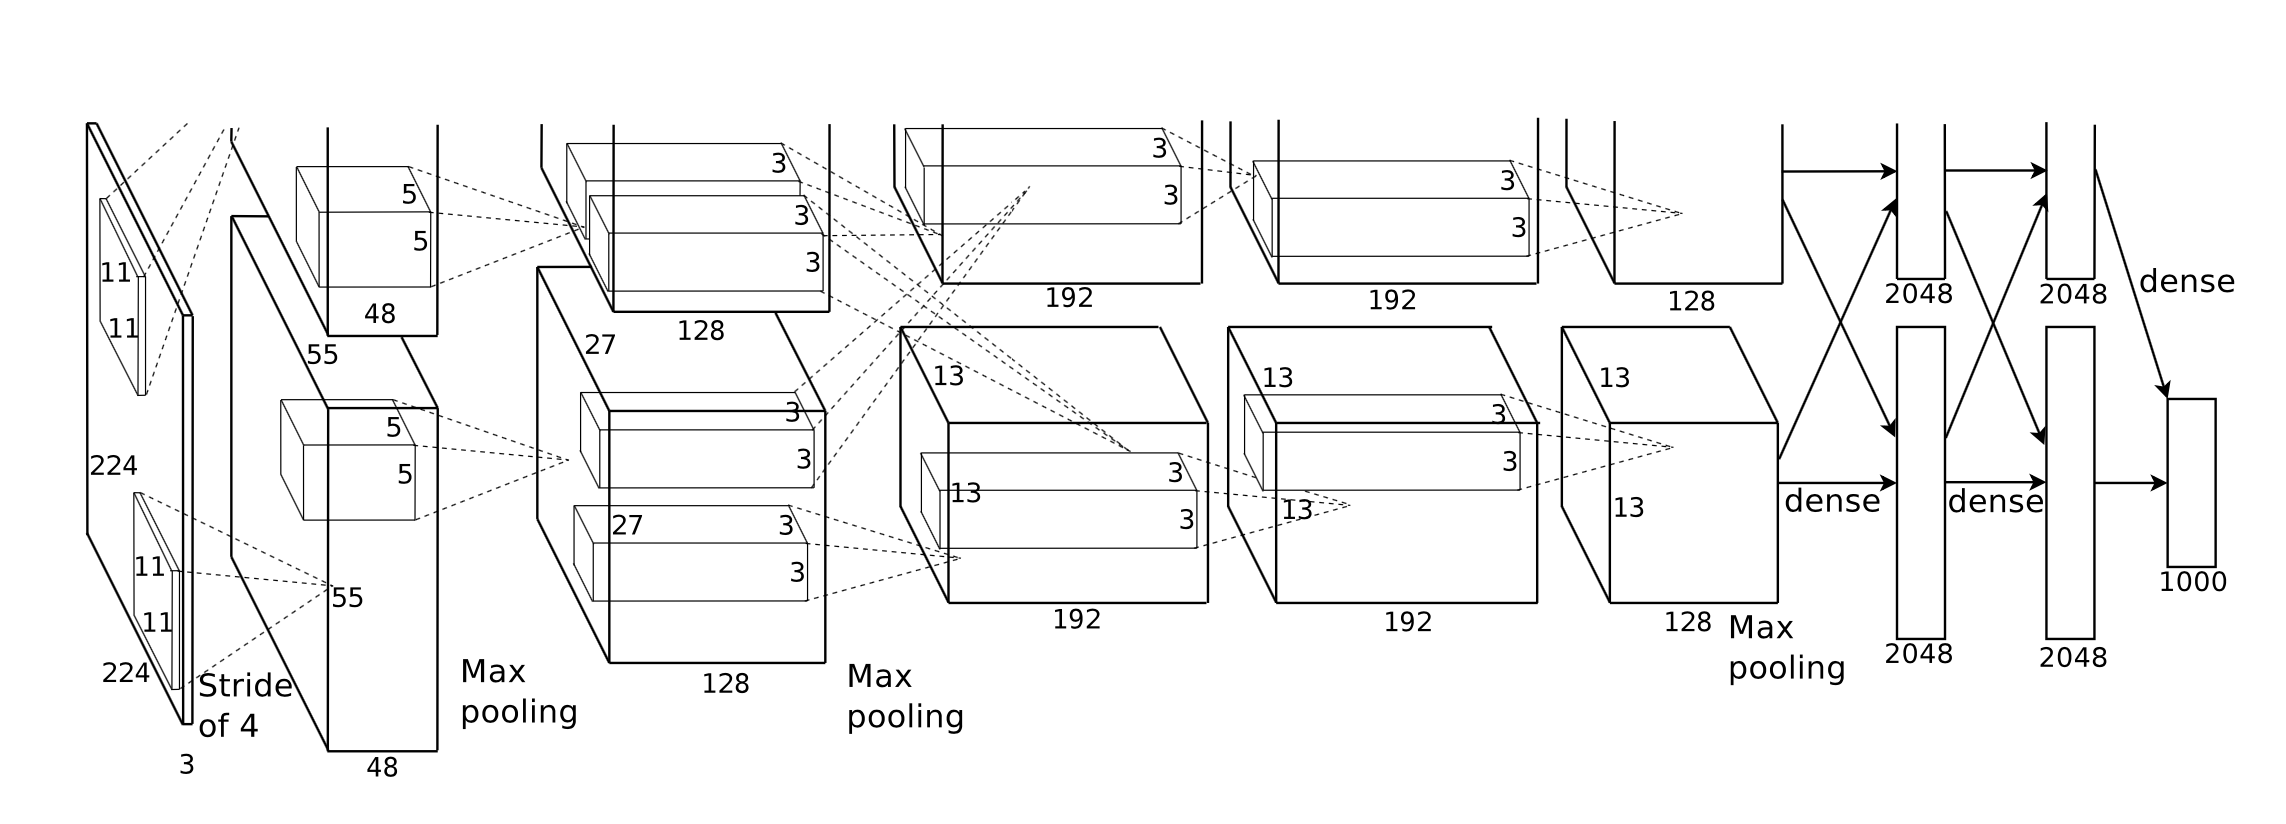
\includegraphics[totalheight=5cm]{imagenet}
    \caption{Imagenet architecture \protect\cite{imagehinton}}
    \label{fig:imagenet}
\end{figure}
They solve overfitting using (1) data augmentation which artificially enlarges the data set using transformations on images and (2) applying dropout where they set the output of each hidden neuron to zero with 0.5 probability. These dropped neurons do not contribute to the forward pass and the backpropagation and the model learns more robust features.
One weakness of this paper is not declaring the decision behind the parameters of the neural network architecture. They also do not provide numerical results for the effects of different dropout probabilities. However, this deep neural network would not work with our data set. Our work complements this by adding a neural network for text classification as well and we suspect it will perform better in the case where image data is missing but we have the HTML of the webpage.
The authors of ~\cite{nipsandrewng} have introduced an extension to convolutional neural networks (CNN) called Tiled CNNs. Rather than all weights being equal, these networks only require hidden units positioned k steps of each other to have equal weights which will lead to learning more complex range of invariances. 
They also use an unsupervised learning algorithm that learns features from unlabeled image patches called Topographic ICA (TICA). They show that TICA pretraining for Tiled CNNs performs well on object recognition. We explain in the future works section, how this work can be integrated into our proposed network. However, a weakness of this paper is that they experiment on a limited number of data sets.

Authors in ~\cite{icml_unsupervised} show that one can use unlabeled data to build high-level, class-specific feature detectors. This will address the challenge of obtaining large labeled data sets. (Practically, this provides an inexpensive way to develop features from unlabeled data.) This work extends the prior work such as using autoencoders for learning low-level features such as "edge" detectors and aims to capture complex invariances. They use a large data set of 200x200 images and feed it into a deep autoencoder with pooling and local contrast normalization. Local receptive fields which indicate that each feature in the autoencoder can connect to a small region of the lower layer in order to scale the autoencoder to large images. Local L2 pooling and local contrast normalization are used to achieve invariance to local deformations. As our data set only contains labeled data we have not used this model but, we will discuss how we can integrate this work with ours in the future works section.



\subsection{Text Classification}

There exists a myriad of publications on text classification. The goal of text classification is to assign free-text documents to predefined categories. In ~\cite{convtext}, authors show that using a convolutional neural network on top of a pre-trained word vector performs well on sentence-level classification tasks. They train a CNN with a single layer of convolution on top of word vectors that are pre-trained on 100 billion words of Google News. From the obtained results, they suggest that using pre-trained vectors are universal feature extractors. Their model's architecture is shown in Fig 2. The structure of our proposed text classification neural network is inspired by this works network. However, our proposed network also receives an image as input while this work only concentrates on text.
In their model a sentence of length $n$ is represented as: $x_{1:n} = x_1 \oplus x_2 \oplus ... \oplus x_n$ and $x_i$ is the k-dimensional word vector for the i-th word. They apply a convolutional operation to a window of $h$ words to produce a new feature. $c_i = f(w\cdot x_{i:i+h-1} + b)$ where $f$ is a non-linear function. Therefore a feature map $c = [c_1, c_2, ...,c_{n-h+1}]$ is constructed, after this a max pooling operation is applied over this feature map where it outputs $\hat{c} = max(c)$ capturing the most important features for each feature map. These features are then passed to a fully connected  layer. The output of the softmax layers is the probability distribution over labels. The model uses multiple filters with different window sizes to obtain multiple features. Regularization is applied by using dropout on the output of the max pooling layer. One of their strong points is performing experiments using several variants of the model. For example comparing the result of CNN with static pre-trained vectors, and CNN with randomly initialized words vectors on multiple data sets. This deep neural network would not also work with our data set because it contains text in addition to images. Our work complements this by adding a neural network for image classification as well and will presumably perform better in the case where text data is missing but we have the image of the webpage.

The authors of ~\cite{nips_text} explore empirical results on the use of character-level CNNs for text classification. In other words, they treat text as a kind of raw signal at character level and apply one-dimensional CNNs to it. Their model takes a sequence of encoded characters as input. The sequence of characters is transformed to a sequence of m sized "one-hot" encoding vectors with fixed length $l_0$. Characters exceeding length $l_0$ are ignored and characters not in the alphabet are set to all-zero vectors. This model works on a set of 70 characters. Their model shown in Fig3, consists of 2 CNNs which both have 6 convolutional layers and 3 fully connected with dropout probability 0.5. We also use this dropout approach in our proposed network. One strong aspect of this paper is applying data augmentation using thesaurus to control generalization error by replacing words by their synonyms. They compare their results to word-based CNN approach described in ~\cite{convtext} as well as traditional text classification models such as bag-of-means on word embeddings. They conclude that the model performance depends on various factors such as data set size and choice of alphabet and show that character-level CNN could work for text classification without needing words. The weakness of their paper is that they do not provide a clear explanation of their model.
Furthermore, a work done by ~\cite{nn_survery}  perform a survey on neural network models from the perspective of natural language processing research. Specifically related to our work are their discussion on convolutional neural networks and the use of word embeddings for representing each feature as a vector in a low dimensional space. According to ~\cite{} convolutional networks with pooling layers perform well in classification tasks. The strong point of this work that it does a comprehensive study on different aspects of neural network models for natural language processing. However, it does not provide sufficient details about each approach. We have designed our text classification neural network while having in mind that  CNNs are to be integrated into a larger network in order to be useful.
\subsection{block page Detection}
~\parencite{imc14_phillipa} propose length differences between a censored page and its uncensored counterpart as a heuristic, 
relying on the idea that blocked pages usually shorter than the original page. However, this approach fails to distinguish server errors from block pages and connection errors. Whereas, our model is designed to distinguish them.
We did not find research on blocked page detection in the field of machine learning, however, machine learning techniques have been used for detecting website defacements by ~\parencite{meerkat}. The structure of their deep neural network was inspired by work from~\parencite{imagehinton}, \parencite{nipsandrewng}, and ~\parencite{icml_unsupervised}.


\clearpage
\section{Methodology}
In this section, we describe the architecture of our convolutional neural network for classifying webpages. Our model consists of two parts that run in parallel. First, the CNN for image classification and secondly, the CNN for text classification. We will describe each of these CNNs and how they interact with each other. We implement our neural network in Python using the tensorflow library.

\subsection{Image Neural Network}
The design of our image classification convolutional neural network is inspired by ~\cite{imagehinton} and consists of a total 5 layers. More specifically, the first three layers are convolutional layers and the final two are fully connected layers. Since we have four categories, the output of the last fully connected layer is given as input to a 4-way softmax function shown in ~\ref{softmax} which predicts the class labels. We use the softmax cross-entropy described in \ref{crossentropy} as our cost function.
\begin{equation} \label{crossentropy}
\theta_{*} = \argmin_\theta \sum_{n=1} ^{N} -ylog(p)-(1-y)log(1-p)
\end{equation}

According to empirical results the Adam optimization algorithm works better than other stochastic optimization methods. Thusm, we employ the Adams algorithm for optimizing the cost function ~\cite{adam}.The first convolutional layers filters the 160x160x3 input images with 32 kernels of size 16x16x3 with a stride of 4 pixels which means we slide the convolutional filter over the input image by 4 pixels at a time, this will reduce the size of the CNNs output. Further, we want the output of the CNN to have the same size as the input, therefore we apply zero padding where 0 values are added to the edge of the input to preserve the input size. We use the ReLU activation function $f(x) = max(0,x)$ for the outputs of the CNN neurons as it is shown to be faster than the alternative $tanh$ activation function~\cite{imagehinton}. We then apply a 2x2 max-pooling where we select the largest value from each 2x2 window. 
The second and third layers filter the output of their previous layer using 64 kernels of size 8x8x3 and 128 kernels of size 4x4x3 with a stride of 4 pixels, 2x2 max pooling, and ReLU activation functions, respectively. As ~\cite{cnndropout2} has shown that using dropout in convolutional neural networks improve performance, we have also done the same.
Finally, we flatten the output of the third convolutional layer in order to make it suitable as input to the fully connected layers with 128 neurons. In order to avoid overfitting, we apply dropout to our fully-connected layers. Prior work has also shown that using dropout on the last hidden layer of a fully-connected layer reduces the error rate ~\cite{cnndropout}. To be more concise, we set zero the output of each hidden neuron with probability 0.5. By doing this, we make sure that the network is not always using the same neurons and is not getting fitted to the training data. The network's architecture is shown in the top part of 
~\ref{fig:cnn}. The full network structure is available in the appendix.

\begin{equation}
  \label{softmax}
  P(y=j | x) = \frac{\exp(x^T w_j)}{\sum^{K}_k=1 \exp(x^T w_k))},
\end{equation}

\subsection{Text Neural Network}
The design of our text classification CNN is inspired by ~\cite{convtext}. Similar to our image classification neural net, it consists of a total 5 layers, with the first three being convolutional networks and the rest being fully connected layers. We need to apply some pre-processing on our HTML data before we can input them to the network. First, we separate the <body> of the HTML pages then we only consider the first 200 words of the body $doc=[w_1,w_2,...w_{200}]$. In order to turn these words into features, we use pre-trained word vectors from GloVe's embedding matrix which contains 300-dimensional vectors for 1.9M words. GloVe is a log-bilinear regression model of word representations ~\cite{glove}. We fetch the vector $v_i$ for the first 200 words in our document from the embedding matrix of GloVe and build $doc = [[v_1],[v_2],...[v_{200}]]$. In the case that the HTML document contains less than 200 words, we pad the final $doc$ with 200-dimensional zero vectors. Therefore, each HTML document will have the shape 1x200x300 with 300 being the number of channels which will be used as input for the convolutional network. The structure of the text CNN is similar to the image classification one and the cost function and optimization algorithm are the same. The first convolutional layer applies a filter to the input using 128 kernels of size 1x4x300 with a stride of 3 pixels. After applying the ReLU function we select the max value within a 1 by 2 window. The mathematical description is as follows:
Every document is the concatenation of the word vectors $doc = [v_1 \oplus v_2 \oplus ... v_{200}]$ and by applying the convolution in windows of size 2 and the ReLU activation function, we will have $c_i = ReLU(w\cdot v_{i:i+2} +b)$ so max pooling will compute the maximum between $c = [c_1, c_2, ... c_{199}]$ which is shown as $\hat{c} = max(c)$.
The second convolutional layer applies a filter using 64 kernels of 1x8x300 with the same max pooling scheme as the previous layer and the third convolutional layer applies a filter with 32 kernels of 1x16x300. ReLU is used as the activation function of all layers and we apply a dropout probability of 0.5. The same flattening process occurs on the output of the third convolutional layer and we go through two fully connected layers with dropout probability of 0.5. The network's architecture is shown in the bottom part of Figure~\ref{fig:cnn}. The full network structure is available in the appendix.
\begin{figure}
\centering
        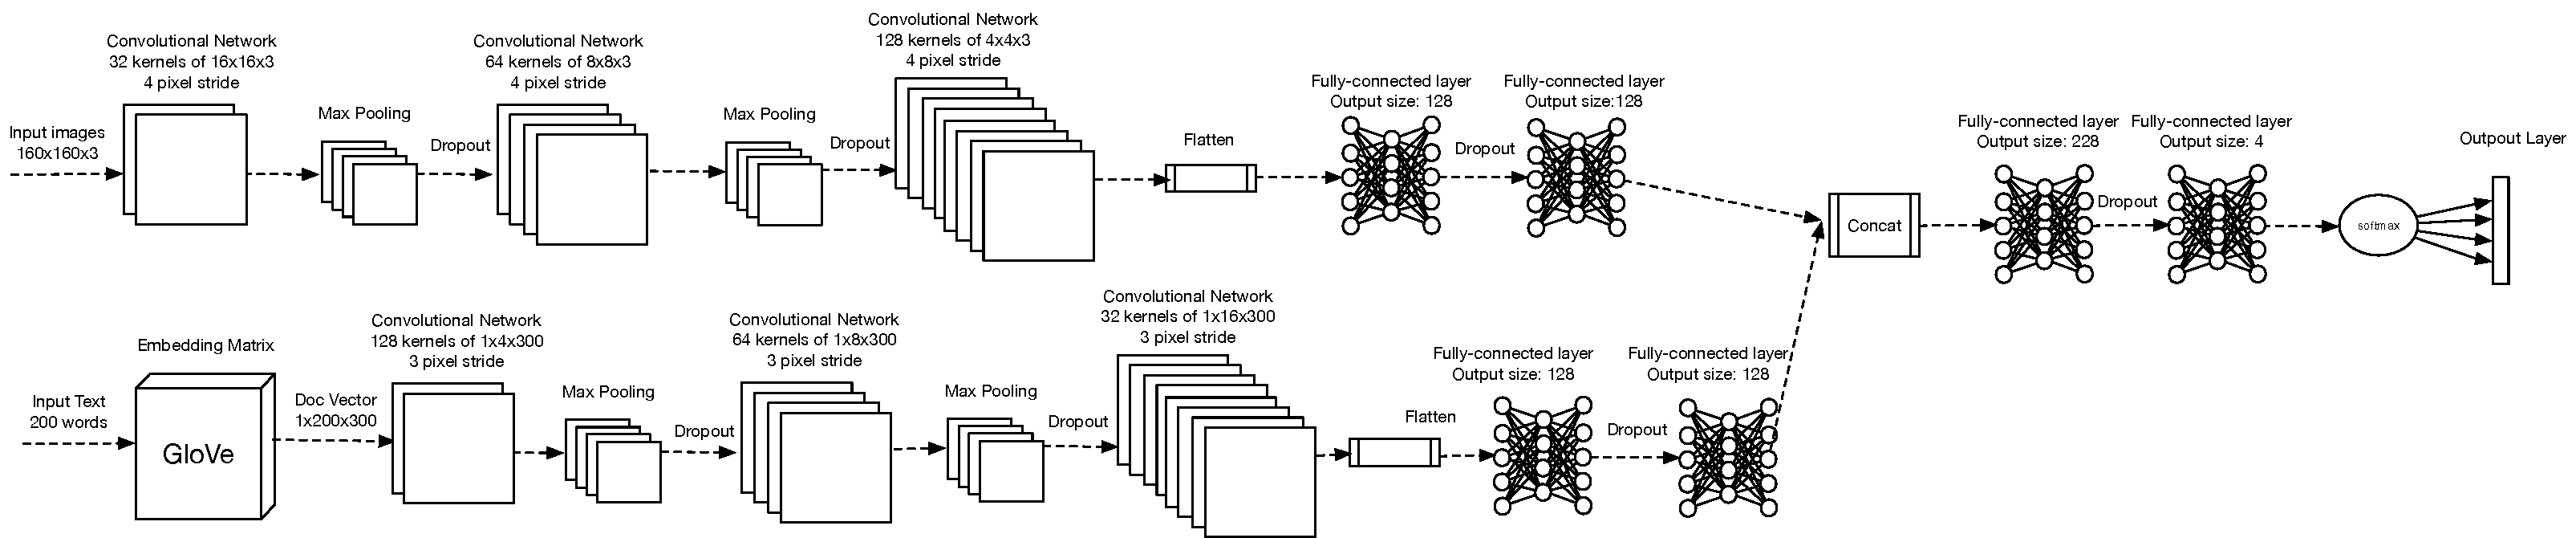
\includegraphics[totalheight=3cm]{Combined}
    \caption{Text classification neural network}
    \label{fig:cnn}
\end{figure}

\subsection{Proposed Neural Network}
Our network as depicted in Figure~\ref{fig:cnn} first receives the HTML document and the Image of the webpage. It then feeds the input into the two separate CNNs and then concats the output of the second fully connected layer of both inputs. We then give that as an input to another fully connected layer and apply a 4-way softmax function to predict the class label.

\section{Data Sets}  \label{datasets}
We use an automated Selenium based web crawler written in Python for collecting screenshots and the HTML documents of Alexa Top 500 websites from a control host and a 145 Tor exit relays located in 23 countries. Our crawls took place dataset consists of 42492 + 86754 number of images and html text documents belonging to 4 categories. Our images have variable-resolutions, therefore we rescale our images to 160x160. We do not crop the center of each image, because many of the server error pages have content shown in the top part of the page. We do not apply pre-processing or data augmentation on our data and use the raw RGB values of the pixels as our image inputs. For the html documents, we take out the <body> section of the page and parse over the first 200 words and provide this as our text inputs.

Glancing at the screenshots we can clearly see four types of pages. (1) the Tor user can access the website like a non-Tor user, we label these pages as \textit{ok}. (2) the Tor user reaches a server error page which we label with \textit{servererr}. (3) the Tor user gets a connection failed or timeout page, we label these as \textit{connectionerr} and finally (4) the Tor user gets a block page or a page containing some form of CAPTCHA which we label as \textit{block}. We use the fact that block pages usually have less length than a normal page ~\cite{imc14_phillipa} and manually label our data set.

\clearpage
\section{Experiments}
In order to evaluate the performance of our proposed model, we compare it using a set of performance metrics with (1) cnn for image classification (2) cnn for text classification (3) prior work for block page detection . We conduct all the experiments on the previously mentioned dataset where we take 80\% of the data randomly as training and set aside the remaining 20\% for the test phase. Out of the 80\% for training, 25\% is also set for validation. Our hypothesis is that the designed cnn should perform better than the cnn for image, the cnn for text classification. The reason being that there are cases where either the image or the text is missing for a data case and our proposed cnn would be more beneficial than a single cnn only focusing on text or image. Finally, since previous techniques for block page detection were only heuristic based and had false positives, our method is designed to classify web pages into 4 distinct classes more accurately. In all experiments, the training batch size, validation batch size and test batch size are 1077 and we will apply X number of epochs.


\subsection{Performance Metrics}
We can not apply accuracy as the performance metric of our prediction, because our dataset is unbalanced. Meaning that the number of \textit{ok} pages is more than the other classes. Hence, we select precision, recall and F1 score as our performance metrics. For a given test set that contains data belonging to four different classes, we get our model's prediction and compute for example, the number of pages correctly predicted as block pages divided by the total pages detected as block pages (precision of block page detection). Further, we measure the number of pages correctly predicted as block pages divided by the number of detected block pages (recall of block page detection). The formulas are also shown in ~\ref{eqn:eqlabel}. These performance metrics have been used to evaluate block page detection in prior work as well ~\cite{imc14_phillipa}.
\begin{align}
\label{eqn:eqlabel}
\begin{split}
 precision = \dfrac{tp}{tp+fp} , \quad 
recall = \dfrac{tp}{tp+fn}, \quad 
f1 = 2 \cdot \dfrac{precision \cdot recall}{precision + recall}
\end{split}
\end{align}


\subsection{Hyperparameters and Training}
We perform a grid search for our hyperparameter tuning. More specifically, we take the learning rate and the size of the first fully-connected layer after the flatten process in the networks as our hyperparameters. For the learning rate, we consider 0.001 and 0.0001 values and for the size of the fully connected layers we consider 256 and 128. Therefore, for each experiment we will consider the effect of these hyperparameters.
\section{Results}
The results of our experiments are listed in table ~\ref{resultifg}

\section{Discussion and Conclusions}
%
%
%
%\subsubsection*{References}
%
%References follow the acknowledgments. Use unnumbered third level heading for
%the references. Any choice of citation style is acceptable as long as you are
%consistent. It is permissible to reduce the font size to `small' (9-point) 
%when listing the references. {\bf Remember that this year you can use
%a ninth page as long as it contains \emph{only} cited references.}
%
%\small{
%[1] Alexander, J.A. \& Mozer, M.C. (1995) Template-based algorithms
%for connectionist rule extraction. In G. Tesauro, D. S. Touretzky
%and T.K. Leen (eds.), {\it Advances in Neural Information Processing
%Systems 7}, pp. 609-616. Cambridge, MA: MIT Press.
%
%[2] Bower, J.M. \& Beeman, D. (1995) {\it The Book of GENESIS: Exploring
%Realistic Neural Models with the GEneral NEural SImulation System.}
%New York: TELOS/Springer-Verlag.
%
%[3] Hasselmo, M.E., Schnell, E. \& Barkai, E. (1995) Dynamics of learning
%and recall at excitatory recurrent synapses and cholinergic modulation
%in rat hippocampal region CA3. {\it Journal of Neuroscience}
%{\bf 15}(7):5249-5262.
%}
\printbibliography
\end{document}